\begin{figure}[htb]
	\centering
	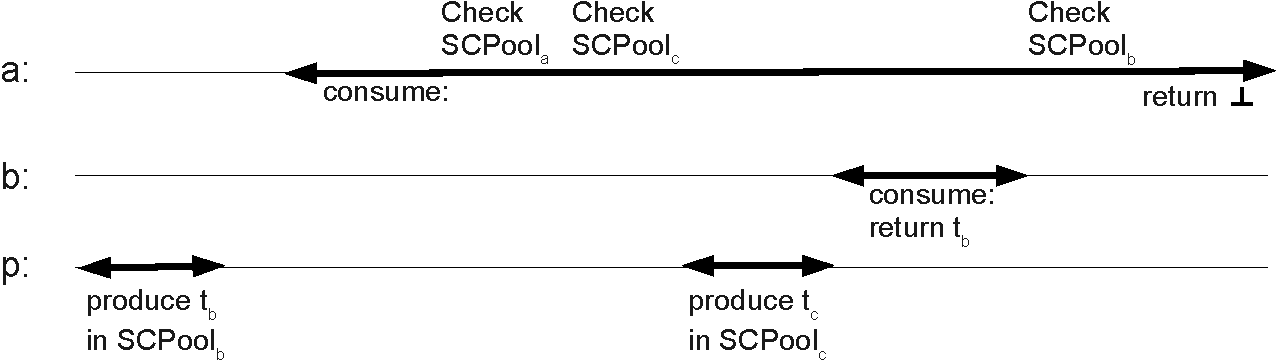
\includegraphics[width=0.7\textwidth]{figures/linearizability-example}
	\caption{\footnotesize{In this scenario $a$, $b$ and $c$ are the only consumers in the system and $p$ is the only producer. Above is a description of the following execution were $a$ trying to get a task: consumer $a$ fails to take a task from its own pool, and starts looking for chunks to steal in other pools. Assume that at this time there is a single non-empty chunk in the system, which is in $b$'s pool. Assume further that $a$ checks $c$'s pool before $b$'s pool and sees that it is empty. At this point a producer adds a task to $c$'s pool and then $b$ takes the last task from its pool before $a$ checks it. Thus, $a$ finds $b$'s pool to be empty, and returns $\bot$. There is no way to linearize this execution, because throughout the execution of the $a$'s operation, the system contained a task.}}
	\label{fig:linearizability-example}
\end{figure}

\paragraph{linearizability}
The algorithm as described in the previous sections is trivially wait-free as all operations of the SALSA pool always return, and the framework only calls a bounded number of those operations. However, this algorithm does not implement a linearizable task pool because an operation may return $\bot$ even when the pool is not empty. 

There are two possible reasons why a consumer may incorrectly return $\bot$. First, the consumer may ``miss'' one task added during its traversal, and another removed during the same traversal. Second, a consumer may miss a task in case a chunk is moved from one pool to another due to stealing. In order to identify these two cases, we add to each pool special counter \emph{emptyCount}, which is increased every time a chunk is reclaimed or stolen (i.e., every time a chunk is removed from the pool).
See the example in Figure~\ref{fig:linearizability-example}.

we now describe a way to make our algorithm linearizable which makes it only lock-free. 
We change the framework of section \ref{sec:system} so that a new function {\bf checkEmpty()} is called whenever a consumer fails to retrieve tasks from its pool and all other pools. This function ensures that $\bot$ is returned only if there is a time when there are no tasks in the system. If {\bf checkEmpty()} finds that the pool is not empty, the consumer restarts its operation. The {\bf checkEmpty()} function works as follows: the consumer traverses all the chunk lists of all SALSA pools in the system, to make sure that no tasks are present. After checking a pool, it reads its value of the \emph{emptyCount}. The consumer repeats this traversal $|consumers|$ times, where in all traversals except the first, it checks that the \emph{emptyCount} value is equal to the value it saw in the first traversal, i.e., that no chunks were moved during the traversal. The reason the consumer makes $|consumers|$ traversals is that other consumers may already stole or removed chunks but did not yet change \emph{emptyCount} and therefore their operations were not detected by the consumer. Since there may be up to $|consumers-1|$ pending operations by other consumers, it is guaranteed that after $|consumers|$ traversals in which no chunks were seen and the \emph{emptyCount} did not change, in one of the traversals the system contains no tasks, and therefore it is safe to return $\bot$. This method is similar to the one used in Concurrent Bags~\cite{Sundell:2011:LAC:1989493.1989550}. However, while our method requires a single fetch-and-increment operation per-steal and per-chunk, their operation requires an additional write on every produce operation, and a CAS operation for every empty chunk encountered in the traversal.

\paragraph{Lock-freedom}
This approach does not guarantee that a consumer will finish its operation. For example, in case the consumer's pool is empty, and its steal operation always fails even when the system contains chunks, this consumer does not make progress. Nevertheless, the system is lock-free, i.e., there always exists some consumer that makes progress. Since a consumer either returns a task or keeps attempting to steal tasks, lock-freedom follows immediately from the following claim:

\begin{claim}
\label{claim:lock-free}
If a consumer fails in $c$ steal attempts from non-empty pools, where $c$ is the number of consumers in the system, then it is guaranteed that at least one consumer in the system returns a task during that time. 
\end{claim}
The proof for this claim is described in Appendix \ref{appendix:lock-freedom}.